\documentclass[letterpaper, 11pt]{article}
\usepackage{nopageno} % For removing page numbers
\usepackage[utf8]{inputenc}
\usepackage{color, colortbl} % For table coloring
\usepackage{titling} % For positioning of title preamble
\usepackage[margin=0.75in]{geometry} % For margin width setting
\usepackage{comment} % For block commenting
\usepackage{float} % For table positioning
% For math equation formatting
\usepackage{amsmath, amssymb, amsfonts}
\newcommand{\PMod}[1]{\ (\mathrm{mod}\ #1)}
\newcommand{\Mod}[1]{\ \mathrm{mod}\ #1}
\usepackage{parskip} % For automatic paragraph spacing/formatting
\usepackage{relsize} % For increased math mode font sizing
% For code blocks
\usepackage[dvipsnames,table]{xcolor}
\usepackage[most]{tcolorbox}
\usepackage{lmodern}
\renewcommand{\ttdefault}{lmtt}
\usepackage{listings, minted}
\lstset{
    basicstyle=\ttfamily\footnotesize,
    keepspaces=false,
    showstringspaces=false,
    keywordstyle=\color{blue},
    commentstyle=\sffamily\itshape\color{Green}\scriptsize,
    stringstyle = \color{red},
    breaklines=true,
    breakatwhitespace=false,
    tabsize=2
}
\tcbset{
    colback=gray!5!white,
    colframe=gray!75!black,
    boxsep=5pt,
}
\setlength{\extrarowheight}{2pt}
\usepackage{titlesec} % Custom styling for section titles
\titleformat{\section}
  {\normalfont\LARGE\bfseries}{\thesection}{1em}{}
\titleformat{\subsection}
  {\normalfont}{\thesection}{1em}{}
% For side-by-side figures
\usepackage{multicol}
\usepackage{makecell}
% For horizontal lists
\usepackage{enumitem, tasks, varwidth}
% For custom page numbers
\usepackage{fancyhdr, lastpage}
\pagestyle{fancy}
\fancyhead{}
\fancyfoot{}
\renewcommand{\headrulewidth}{0pt}
\usepackage[skip=2pt]{caption}
\usepackage{graphicx}
\graphicspath{{../Images/}}

% Move title area to the top of the page
\setlength{\droptitle}{-4em}
\addtolength{\droptitle}{-4pt} 
\renewcommand{\arraystretch}{1.25}
% Disable paragraph indenting
\setlength{\parindent}{0pt}

\usepackage[none]{hyphenat}
\usepackage{times}
\usepackage{soul}

\title{CS430 Homework 2}
\author{Brendan Nguyen}
\date{Due: Wednesday, Mar. 1, 2023}

\begin{document}

\maketitle

\section*{Question 1 (30 points)}

A movie platform database contains information about \textit{authors} (identified by \texttt{authorid}) and information about \textit{books} (identified by \texttt{bookid}). Each book also has a name, a genre, a release year, and a publisher (i.e. publishing company). Authors also have a name, age, phone, and address. Authors write books.

\begin{enumerate}[label={\alph*})]
    \item Draw the ER diagram of this database (as described in the Question 1 statement). Do not use any other constraints.
    \begin{figure}[H]
        \centering
        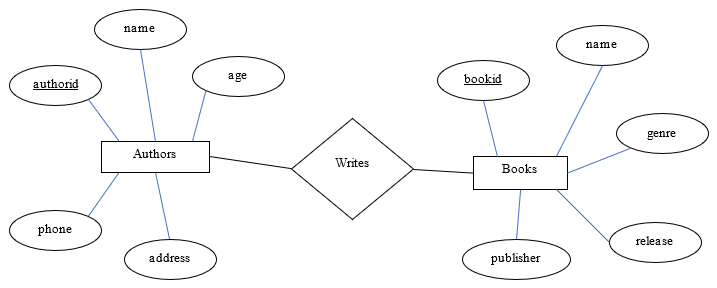
\includegraphics[scale=0.7]{hw2-1a.png}
    \end{figure}
    \item Modify the diagram from a) further to add the constraint that each book must be written by at least one author.
    \begin{figure}[H]
        \centering
        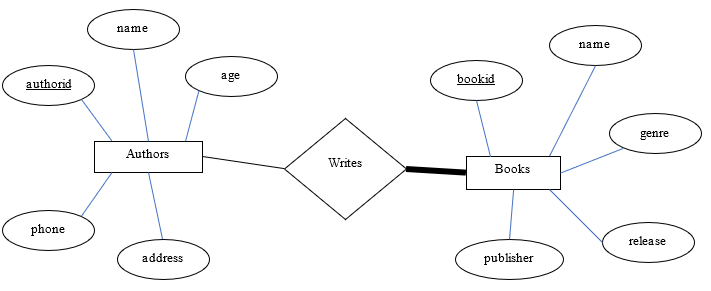
\includegraphics[scale=0.7]{hw2-1b.png}
    \end{figure}
    \item Modify the diagram from b) further to add the constraint that each author must write at most one book.
    \begin{figure}[H]
        \centering
        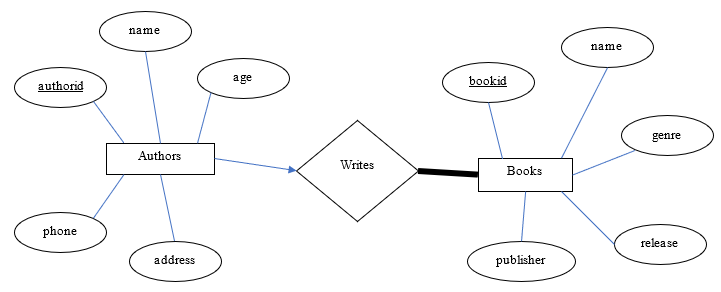
\includegraphics[scale=0.7]{hw2-1c.png}
    \end{figure}
    \item Modify the diagram from c) further to add the constraint such that each book must be written by exactly one author.
    \begin{figure}[H]
        \centering
        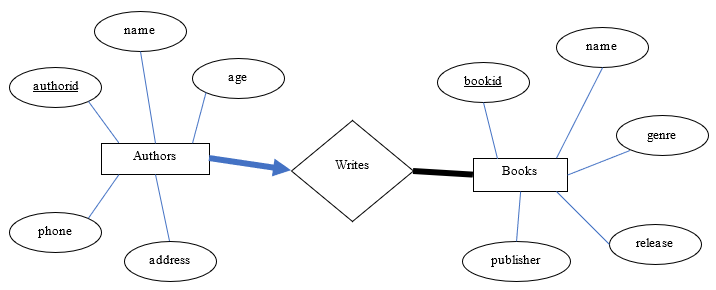
\includegraphics[scale=0.7]{hw2-1d.png}
    \end{figure}
    \item Modify the diagram from d) further such that each author can have multiple phone numbers.
    \begin{figure}[H]
        \centering
        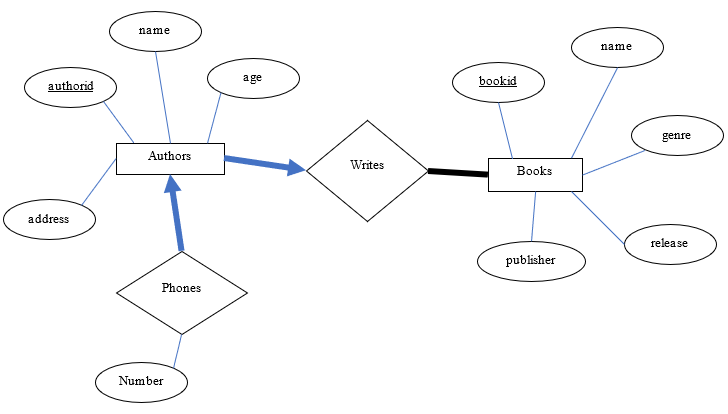
\includegraphics[scale=0.7]{hw2-1e.png}
    \end{figure}
    \item Modify the diagram from e) further such that each author must have at least one phone number.
    \begin{figure}[H]
        \centering
        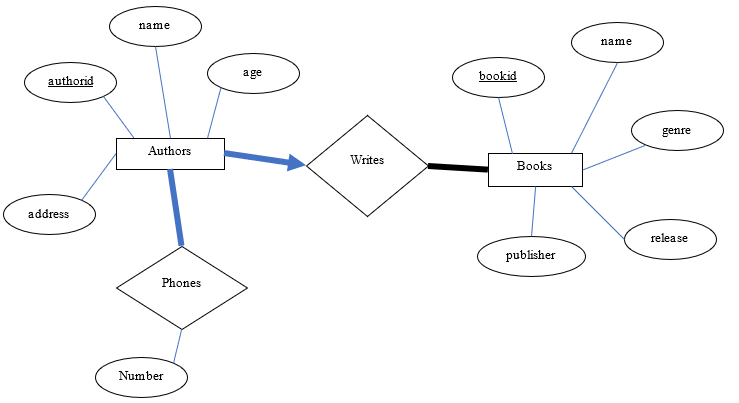
\includegraphics[scale=0.7]{hw2-1f.png}
    \end{figure}
\end{enumerate}

\section*{Question 2 (30 points)}

Given a database that stores information about \textit{Persons} (identified by \texttt{id}) and \textit{Countries} (identified by \texttt{countryname}). A country also has a capital, a president, and a continent. A person also has a first name, a last name, date of birth (dob). Persons visit Countries.\\
NOTES: the ER diagram should strictly follow the notations used in class. No other notations will receive any points.

\begin{enumerate}[label={\alph*})]
    \item Draw the ER diagram that describes this database. Do not add any additional constraints.
    \begin{figure}[H]
        \centering
        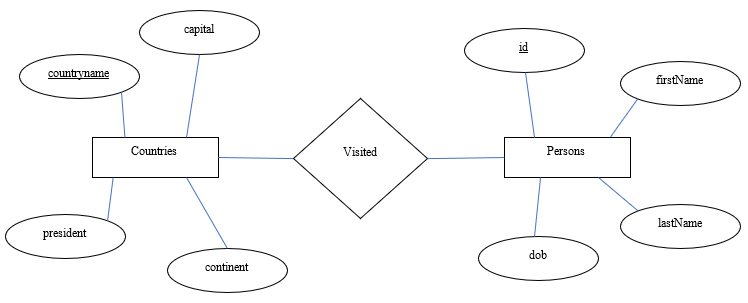
\includegraphics[scale=0.7]{hw2-2a.png}
    \end{figure}
    \item Write the database schema for this ER diagram.

    \begin{itemize}
        \item \textit{Countries} (\ul{\texttt{countryname}: string}, \texttt{capital}: string, \texttt{president}: string, \texttt{continent}: string)
        \item \textit{Persons} (\ul{\texttt{id}: int}, \texttt{firstName}: string, \texttt{lastName}: string, \texttt{dob}: date)
        \item \textit{Visited} (\ul{\texttt{id}: int, \texttt{countryname}: string})
    \end{itemize}
    
    \item Write the SQL \texttt{CREATE TABLE} statements for all tables identified for this database.\\
    The create statements have to work when ran against the Oracle database.\\
    The create statements have to be written in an order such that if executed in that order will not cause any error.
\begin{tcolorbox}
    \begin{lstlisting}[language=SQL]
CREATE TABLE Countries (
    countryname VARCHAR(20) PRIMARY KEY,
    capital VARCHAR(20),
    president VARCHAR(20),
    continent VARCHAR(20)
);

CREATE TABLE Persons (
    id NUMBER(9) PRIMARY KEY,
    firstName VARCHAR(20),
    lastName VARCHAR(20),
    dob DATE
);

CREATE TABLE Visited (
    id NUMBER(9),
    countryname VARCHAR(20),
    PRIMARY KEY(id, countryname),
    FOREIGN KEY(id) REFERENCES Persons,
    FOREIGN KEY(countryname) REFERENCES Countries
);
    \end{lstlisting}
    \end{tcolorbox}
    
    \item Write the SQL statement to update the table \textit{Persons} to add two new columns: city and state.
    \begin{tcolorbox}
    \begin{lstlisting}[language=SQL]
ALTER TABLE Persons ADD (
    city VARCHAR(50),
    state VARCHAR(50)
);
    \end{lstlisting}   
    \end{tcolorbox}
    
    
    \item Write the SQL statements to remove these three tables from the database. Write the statements in an order such that if executed in that order no error will occur.
    \begin{tcolorbox}
    \begin{lstlisting}[language=SQL]
DROP TABLE Visited;
DROP TABLE Persons;
DROP TABLE Countries;
    \end{lstlisting}
    \end{tcolorbox}
    
\end{enumerate}

\section*{Question 3 (40 points)}

(provide your answers to this in an SQL file)

Given the following schema:
\begin{itemize}
    \item \textit{songs} (\ul{\texttt{songid}: int}, \texttt{title}: string, \texttt{release}: date)
    \item \textit{singers} (\ul{\texttt{singerid}: int}, \texttt{name}: string, \texttt{age}: real, \texttt{city}: string, \texttt{state}: string)
    \item \textit{singsin} (\ul{\texttt{singerid}: int, \texttt{songid}: int})
\end{itemize}

The primary keys are uld in each relation. Relation \textit{singers} contains information about singers. Relation \textit{songs} contain information about songs. Relation \textit{singsin} contains information about singers singing songs.

\begin{enumerate}[label={\alph*})]
    \item Write the SQL statements that create tables \textit{songs}, \textit{singers} and \textit{singsin}. Don’t forget to define the key constraints.
    \item Write the SQL query that extracts all the names of the singers from Boston. Sort the result by name in ascending order.
    \item Write the SQL query that extracts information about the singers and the songs they sing. Each record in the result should contain the name and age of the singer, the title of the song, and the release date of the song. Sort the result by the name of the singers in descending order.
    \item Write the SQL query that finds how many singers from Los Angeles, CA are in the database.
    \item Write the SQL that extracts information about singers whose name ends with the letter ``a". Sort the result by the state of the singers, in descending order.
    \item Write the SQL that extracts the name and state for all singers who played in a song that has a title that contains the word happy. The query should be case insensitive with regard to the case of the letters from the title of the song.
    \item Write an SQL query to extract the name, city, and state of singers that sang a song that was released after Aug 10, 2022.
    \item Write the SQL to extract the names of the oldest songs.
    \item Write the SQL to extract the number of unique singers that sang some songs between Jan 1\textsuperscript{st} 2022 and May 31\textsuperscript{st} 2022 (including these dates).
    \item Write the SQL that extracts the number of songs released in the year 2020.
\end{enumerate}

\end{document}
